\documentclass[11pt,aspectratio=169]{beamer}

\usepackage[T1]{fontenc}
\usepackage{lmodern}
\usepackage{booktabs}
\usepackage{listings}
\usepackage{graphicx}
\usepackage{appendixnumberbeamer}  % total page count excludes the appendix
% -----------------------------------------------------------------------------
% Plain style, shared with the other decks
% -----------------------------------------------------------------------------
% =============================================================================
% Shared slide style for the course.
%
%   % =============================================================================
% Shared slide style for the course.
%
%   % =============================================================================
% Shared slide style for the course.
%
%   \input{../beamer-style}          % from inside a deck's own folder
%
% Plain and typographic: serif text on a white page, dark blue frame titles set
% as text rather than in a coloured bar, a small grey page number, and nothing
% else. Each deck keeps its own diagram, figure and listing colours; this file
% governs only the furniture of the frame.
%
% Requires: xcolor (beamer loads it), and \title set before \titleslide.
% =============================================================================

\usefonttheme{serif}

\definecolor{DarkBlue}{RGB}{0,0,110}
\definecolor{DarkRed}{RGB}{140,0,0}
\definecolor{Grey}{RGB}{90,90,90}

\setbeamercolor{normal text}{fg=black,bg=white}
\setbeamercolor{structure}{fg=DarkBlue}
\setbeamercolor{frametitle}{fg=DarkBlue,bg=white}
\setbeamercolor{title}{fg=black}

\setbeamerfont{frametitle}{series=\bfseries,size=\large}
\setbeamertemplate{navigation symbols}{}
\setbeamertemplate{frametitle}{%
  \vspace{0.35cm}\insertframetitle\par\vspace{-0.15cm}}
\setbeamertemplate{itemize item}{\textbullet}
\setbeamertemplate{itemize subitem}{--}
\setbeamertemplate{enumerate item}{\insertenumlabel.}
\setbeamertemplate{footline}{%
  \hfill\color{Grey}\scriptsize
  \insertframenumber/\inserttotalframenumber\hspace{0.6cm}\vspace{0.25cm}}

% -----------------------------------------------------------------------------
% Section dividers: one plain outline frame at the start of each section,
% with the current section in dark blue and the others in grey.
% -----------------------------------------------------------------------------
% \small, and a measured gap rather than \smallskip, so that a deck with eight
% sections still fits on one outline slide.
\setbeamerfont{section in toc}{size=\small}
\setbeamercolor{section in toc}{fg=Grey}
\setbeamercolor{section in toc shaded}{fg=Grey}
% Beamer fades unvisited sections to 20% by default, which disappears on a
% projector. 45% still reads as secondary but stays legible from the back.
\setbeamertemplate{section in toc shaded}[default][45]
\setbeamertemplate{section in toc}{%
  \inserttocsectionnumber.\quad\inserttocsection\par\smallskip}

\AtBeginSection[]{%
  \begin{frame}{Outline}
    \vspace{0.4em}
    \tableofcontents[currentsection,
                     sectionstyle=show/shaded,
                     subsectionstyle=hide]
  \end{frame}}

% -----------------------------------------------------------------------------
% The title slide, and the divider that opens an appendix. Identical in every
% deck, so define them once.
% -----------------------------------------------------------------------------
\newcommand{\titleslide}{%
  \begin{frame}[plain]
    \vfill
    \centering
    {\LARGE\inserttitle}
    \vfill
  \end{frame}}

\newcommand{\dividerslide}[1]{%
  \begin{frame}[plain]
    \vfill\centering{\LARGE #1}\vfill
  \end{frame}}
          % from inside a deck's own folder
%
% Plain and typographic: serif text on a white page, dark blue frame titles set
% as text rather than in a coloured bar, a small grey page number, and nothing
% else. Each deck keeps its own diagram, figure and listing colours; this file
% governs only the furniture of the frame.
%
% Requires: xcolor (beamer loads it), and \title set before \titleslide.
% =============================================================================

\usefonttheme{serif}

\definecolor{DarkBlue}{RGB}{0,0,110}
\definecolor{DarkRed}{RGB}{140,0,0}
\definecolor{Grey}{RGB}{90,90,90}

\setbeamercolor{normal text}{fg=black,bg=white}
\setbeamercolor{structure}{fg=DarkBlue}
\setbeamercolor{frametitle}{fg=DarkBlue,bg=white}
\setbeamercolor{title}{fg=black}

\setbeamerfont{frametitle}{series=\bfseries,size=\large}
\setbeamertemplate{navigation symbols}{}
\setbeamertemplate{frametitle}{%
  \vspace{0.35cm}\insertframetitle\par\vspace{-0.15cm}}
\setbeamertemplate{itemize item}{\textbullet}
\setbeamertemplate{itemize subitem}{--}
\setbeamertemplate{enumerate item}{\insertenumlabel.}
\setbeamertemplate{footline}{%
  \hfill\color{Grey}\scriptsize
  \insertframenumber/\inserttotalframenumber\hspace{0.6cm}\vspace{0.25cm}}

% -----------------------------------------------------------------------------
% Section dividers: one plain outline frame at the start of each section,
% with the current section in dark blue and the others in grey.
% -----------------------------------------------------------------------------
% \small, and a measured gap rather than \smallskip, so that a deck with eight
% sections still fits on one outline slide.
\setbeamerfont{section in toc}{size=\small}
\setbeamercolor{section in toc}{fg=Grey}
\setbeamercolor{section in toc shaded}{fg=Grey}
% Beamer fades unvisited sections to 20% by default, which disappears on a
% projector. 45% still reads as secondary but stays legible from the back.
\setbeamertemplate{section in toc shaded}[default][45]
\setbeamertemplate{section in toc}{%
  \inserttocsectionnumber.\quad\inserttocsection\par\smallskip}

\AtBeginSection[]{%
  \begin{frame}{Outline}
    \vspace{0.4em}
    \tableofcontents[currentsection,
                     sectionstyle=show/shaded,
                     subsectionstyle=hide]
  \end{frame}}

% -----------------------------------------------------------------------------
% The title slide, and the divider that opens an appendix. Identical in every
% deck, so define them once.
% -----------------------------------------------------------------------------
\newcommand{\titleslide}{%
  \begin{frame}[plain]
    \vfill
    \centering
    {\LARGE\inserttitle}
    \vfill
  \end{frame}}

\newcommand{\dividerslide}[1]{%
  \begin{frame}[plain]
    \vfill\centering{\LARGE #1}\vfill
  \end{frame}}
          % from inside a deck's own folder
%
% Plain and typographic: serif text on a white page, dark blue frame titles set
% as text rather than in a coloured bar, a small grey page number, and nothing
% else. Each deck keeps its own diagram, figure and listing colours; this file
% governs only the furniture of the frame.
%
% Requires: xcolor (beamer loads it), and \title set before \titleslide.
% =============================================================================

\usefonttheme{serif}

\definecolor{DarkBlue}{RGB}{0,0,110}
\definecolor{DarkRed}{RGB}{140,0,0}
\definecolor{Grey}{RGB}{90,90,90}

\setbeamercolor{normal text}{fg=black,bg=white}
\setbeamercolor{structure}{fg=DarkBlue}
\setbeamercolor{frametitle}{fg=DarkBlue,bg=white}
\setbeamercolor{title}{fg=black}

\setbeamerfont{frametitle}{series=\bfseries,size=\large}
\setbeamertemplate{navigation symbols}{}
\setbeamertemplate{frametitle}{%
  \vspace{0.35cm}\insertframetitle\par\vspace{-0.15cm}}
\setbeamertemplate{itemize item}{\textbullet}
\setbeamertemplate{itemize subitem}{--}
\setbeamertemplate{enumerate item}{\insertenumlabel.}
\setbeamertemplate{footline}{%
  \hfill\color{Grey}\scriptsize
  \insertframenumber/\inserttotalframenumber\hspace{0.6cm}\vspace{0.25cm}}

% -----------------------------------------------------------------------------
% Section dividers: one plain outline frame at the start of each section,
% with the current section in dark blue and the others in grey.
% -----------------------------------------------------------------------------
% \small, and a measured gap rather than \smallskip, so that a deck with eight
% sections still fits on one outline slide.
\setbeamerfont{section in toc}{size=\small}
\setbeamercolor{section in toc}{fg=Grey}
\setbeamercolor{section in toc shaded}{fg=Grey}
% Beamer fades unvisited sections to 20% by default, which disappears on a
% projector. 45% still reads as secondary but stays legible from the back.
\setbeamertemplate{section in toc shaded}[default][45]
\setbeamertemplate{section in toc}{%
  \inserttocsectionnumber.\quad\inserttocsection\par\smallskip}

\AtBeginSection[]{%
  \begin{frame}{Outline}
    \vspace{0.4em}
    \tableofcontents[currentsection,
                     sectionstyle=show/shaded,
                     subsectionstyle=hide]
  \end{frame}}

% -----------------------------------------------------------------------------
% The title slide, and the divider that opens an appendix. Identical in every
% deck, so define them once.
% -----------------------------------------------------------------------------
\newcommand{\titleslide}{%
  \begin{frame}[plain]
    \vfill
    \centering
    {\LARGE\inserttitle}
    \vfill
  \end{frame}}

\newcommand{\dividerslide}[1]{%
  \begin{frame}[plain]
    \vfill\centering{\LARGE #1}\vfill
  \end{frame}}


\definecolor{CodeBG}{RGB}{246,246,246}

\newenvironment{wideitemize}
  {\begin{itemize}\setlength{\itemsep}{10pt}}
  {\end{itemize}}

\lstdefinestyle{code}{
  basicstyle=\ttfamily\scriptsize,
  backgroundcolor=\color{CodeBG},
  frame=none,
  showstringspaces=false,
  columns=fullflexible,
  keepspaces=true,
  upquote=true,
  aboveskip=0.6em,
  belowskip=0.4em,
  keywordstyle=\color{DarkBlue},
  commentstyle=\color{Grey},
  stringstyle=\color{DarkRed}
}
\lstdefinestyle{py}{style=code,language=Python}

\title{Web Scraping for Applied Research}
\date{}
\author{}

\begin{document}

% =============================================================================
\titleslide

% =============================================================================
\begin{frame}{Why scrape}
\begin{wideitemize}
  \item Some information is public, but exists only as web pages.
  \item Job postings state salaries. No standard dataset collects them.
  \item An afternoon of scraping produces a usable dataset.
  \item The same method works for courts, procurement, company registers.
\end{wideitemize}
\end{frame}

% =============================================================================
\begin{frame}{Posted pay avoids a classic problem}
\begin{wideitemize}
  \item Admin data show what each worker is actually paid.
  \item But better workers sort into better jobs, so pay and quality are tangled.
  \item A posted range is attached to the job, before anyone is hired.
  \item It prices the job itself, not the worker who takes it.
\end{wideitemize}
\end{frame}

% =============================================================================
\begin{frame}{Three questions}
\begin{wideitemize}
  \item Several US states now require postings to state a salary range.
  \item The same job is often posted with a single attribute changed.
  \item How much does the posted range change with location?
  \item What is a skill worth?
  \item Is remote work paid for, or discounted?
\end{wideitemize}
\end{frame}

% =============================================================================
\section{Look first}
\begin{frame}{Rule number one}
\begin{wideitemize}
  \item Never write a scraper for a page you have not read.
  \item Find the number on screen first.
  \item Then ask how the page obtained it.
  \item Ten minutes of looking saves an afternoon of guessing.
\end{wideitemize}
\end{frame}

% =============================================================================
\begin{frame}{The board: every job at one firm}
\centering
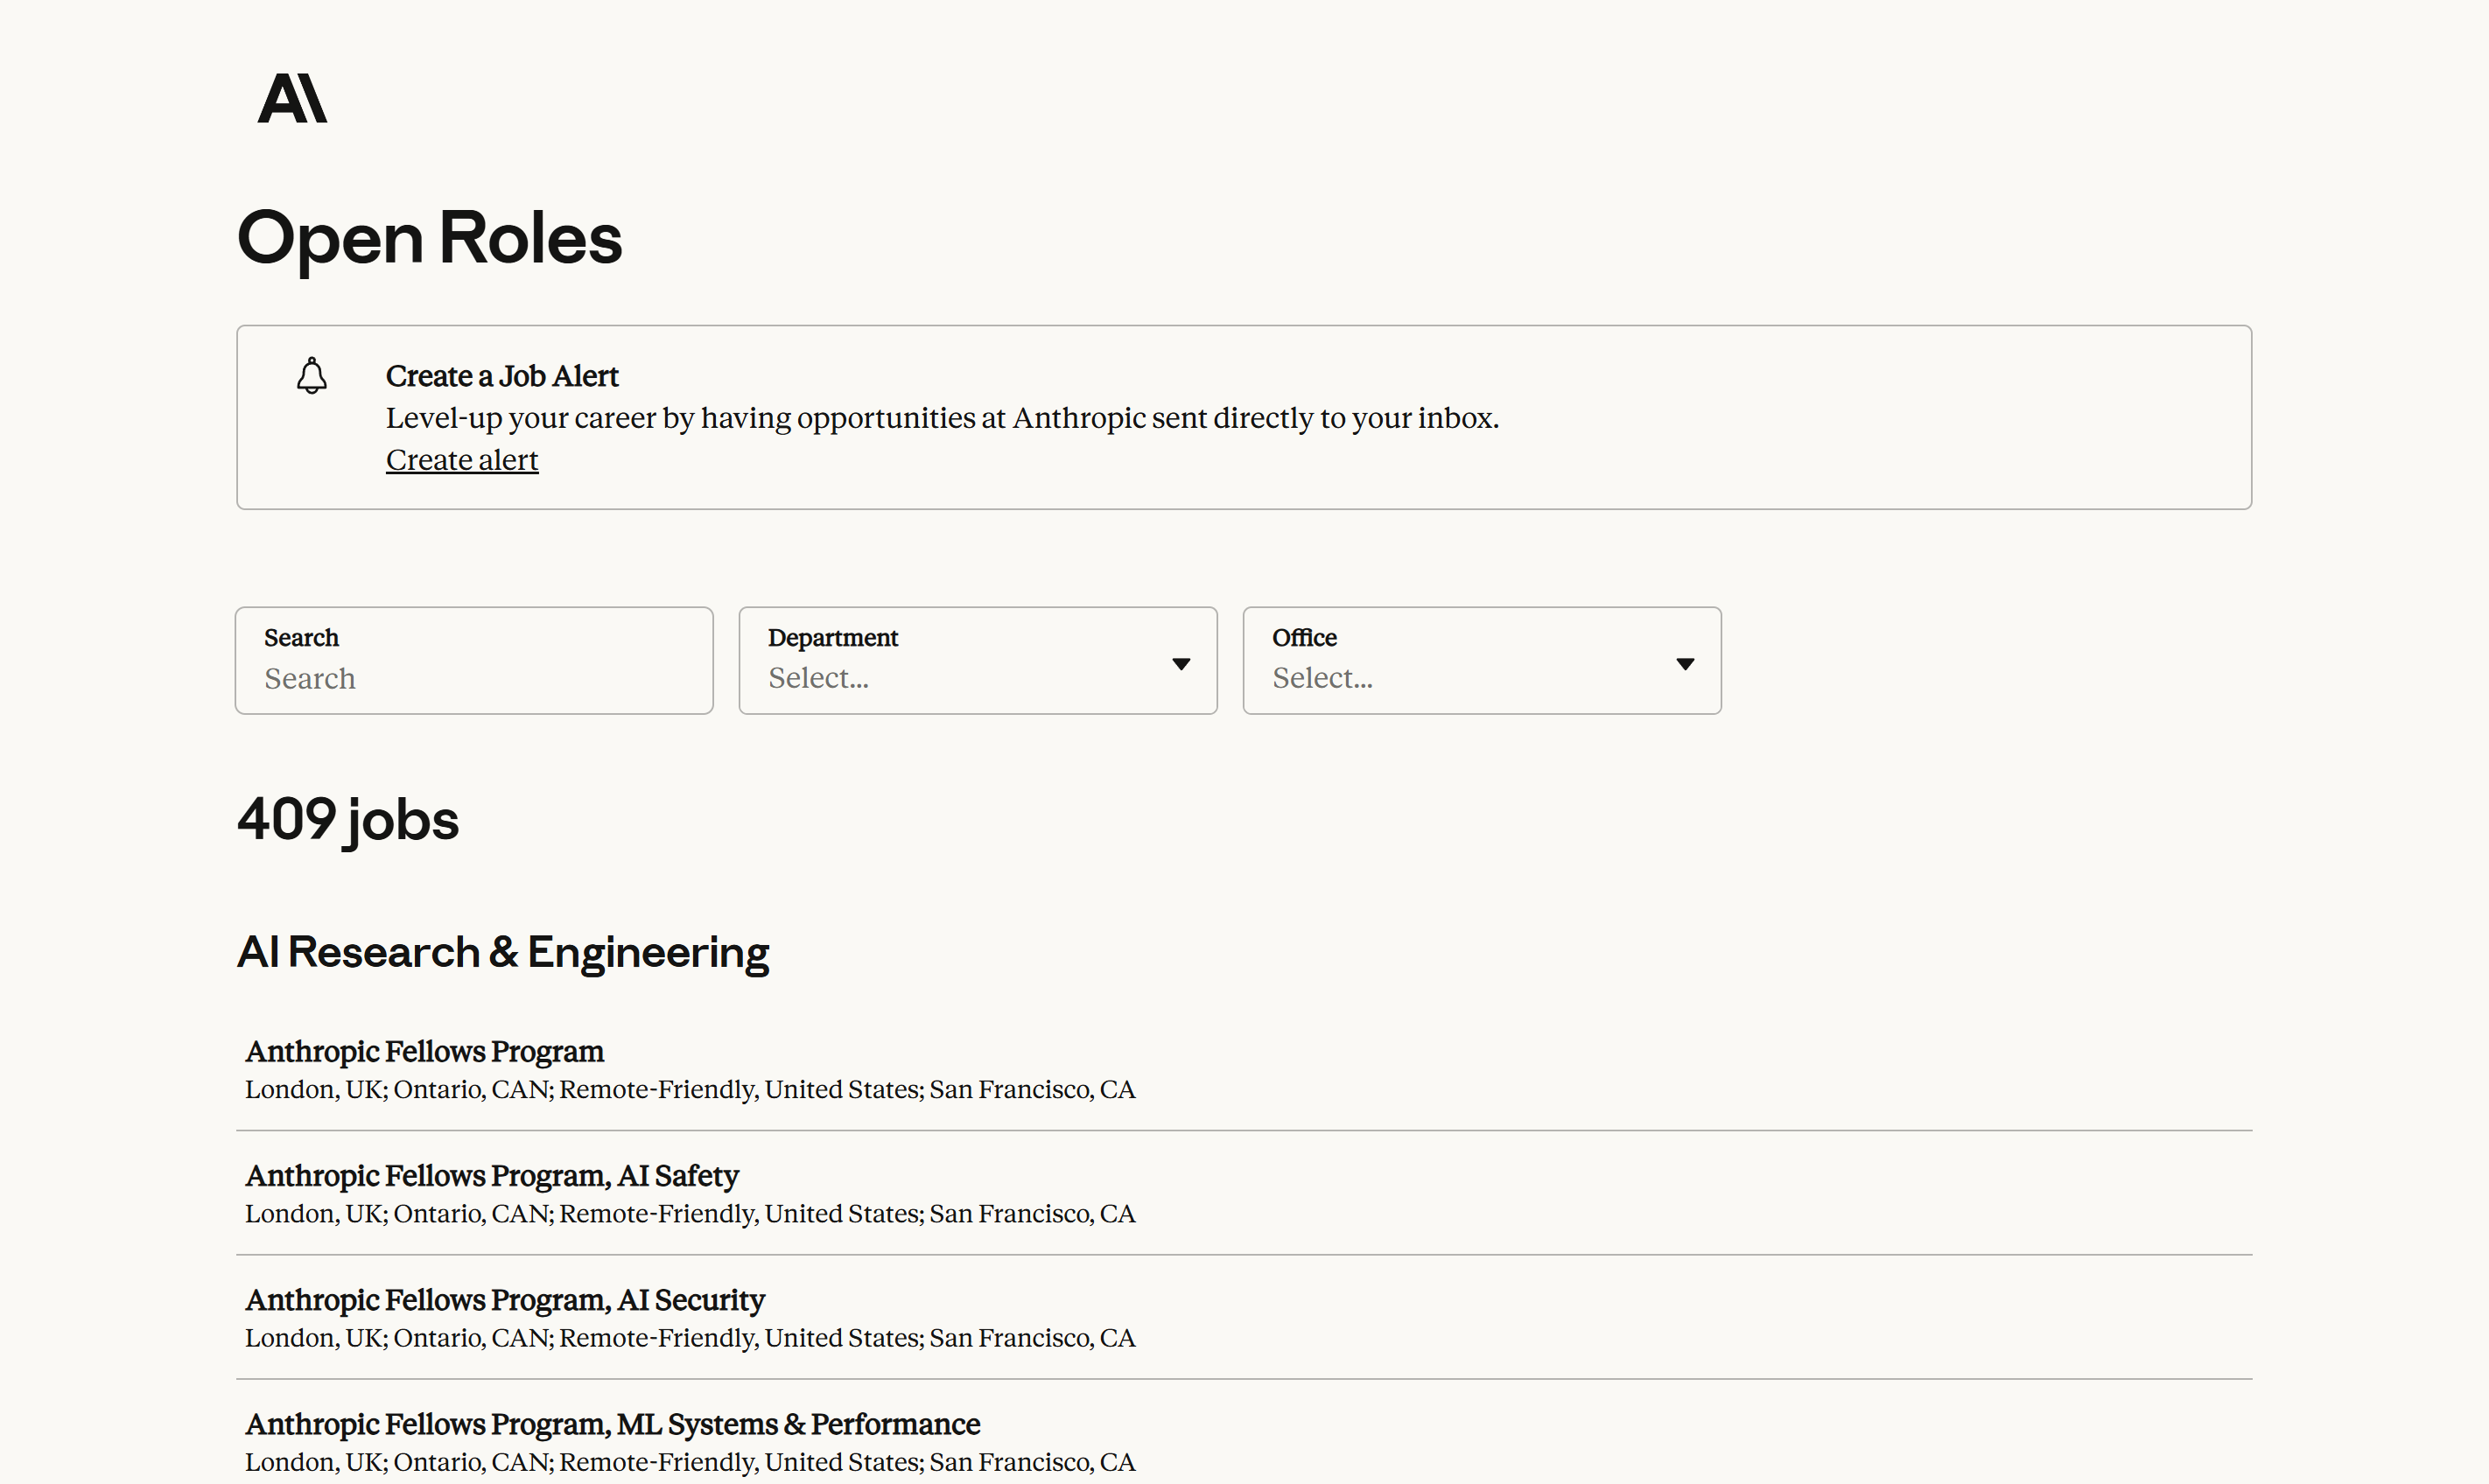
\includegraphics[width=0.78\textwidth,height=0.66\textheight,keepaspectratio]{figs/01_board_page.png}

\vspace{0.3em}
{\footnotesize A list of links. No salaries here.}
\end{frame}

% =============================================================================
\begin{frame}{One posting}
\centering

\includegraphics[width=0.76\textwidth,height=0.70\textheight,keepaspectratio]{figs/02_job_page_top.png}
\end{frame}

% =============================================================================
\begin{frame}{Scroll down: the numbers}
\centering
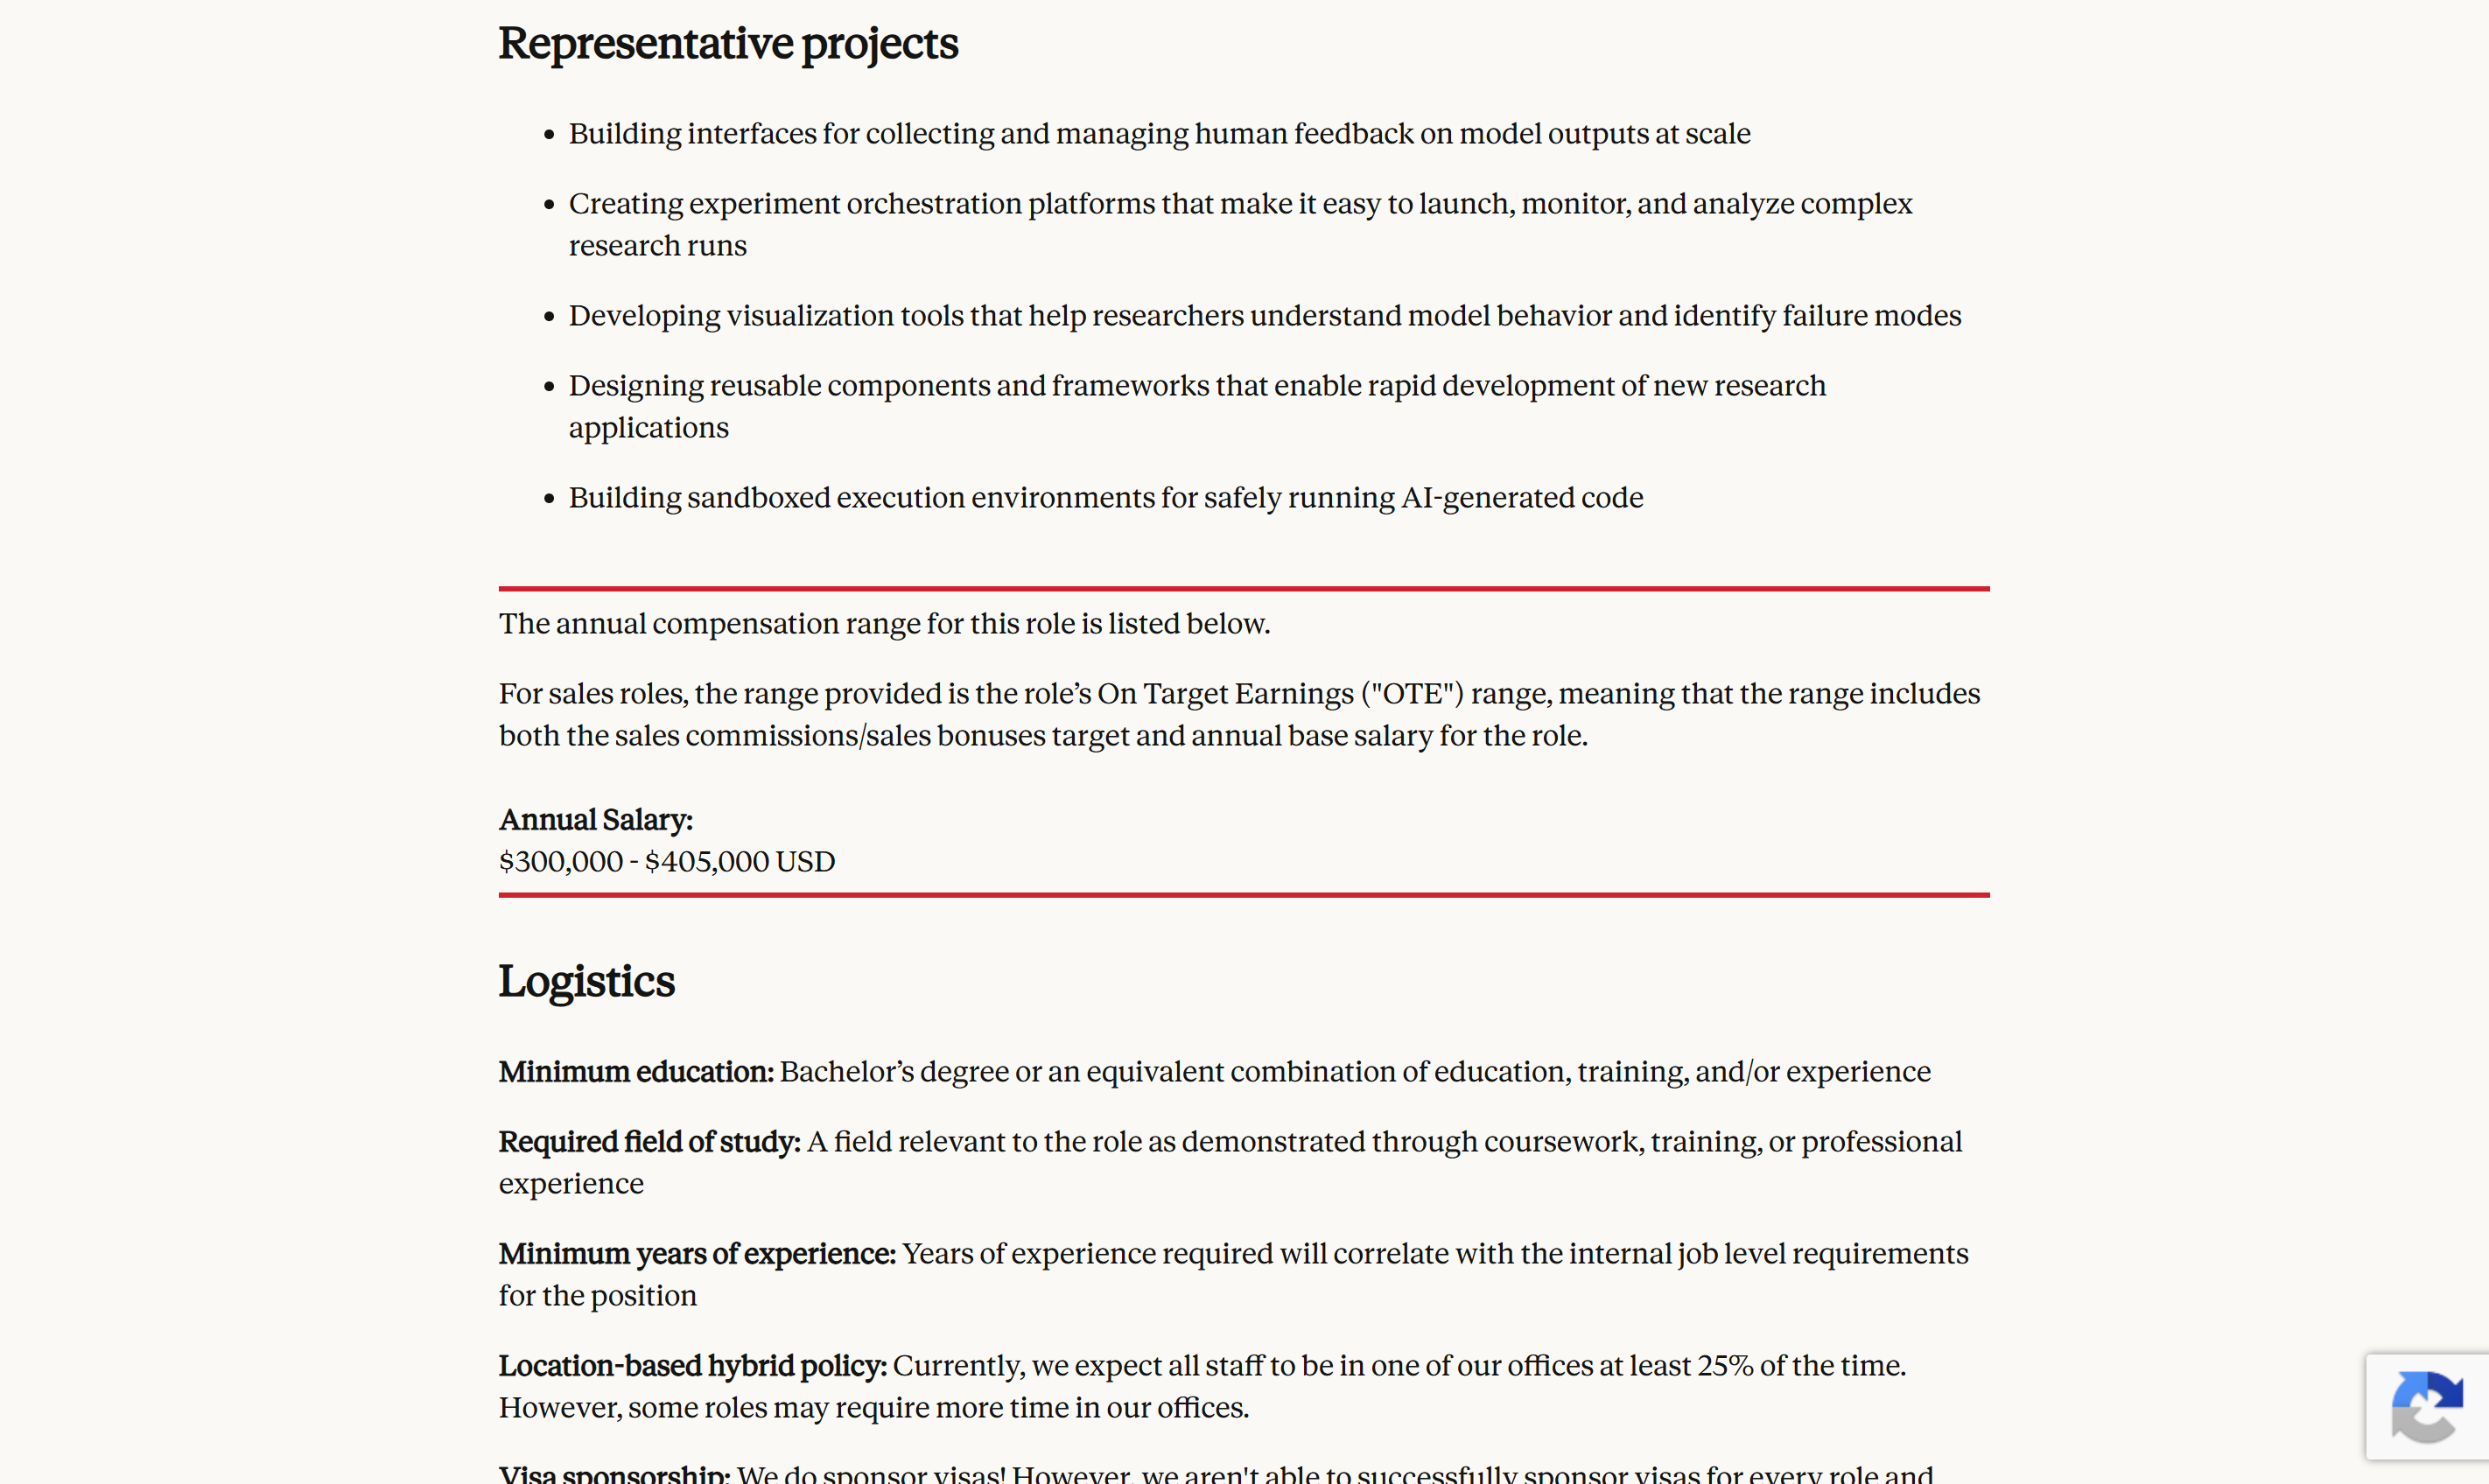
\includegraphics[width=0.70\textwidth,height=0.66\textheight,keepaspectratio]{figs/03_job_page_pay_highlighted.png}

\vspace{0.3em}
{\footnotesize Postings change constantly, so your numbers will differ from these.}
\end{frame}

% =============================================================================
\begin{frame}[fragile]{Where the numbers sit}
\begin{lstlisting}[style=code]
<div class="pay-input">
  <bdi>$300,000</bdi>
  <span>-</span>
  <bdi>$405,000</bdi>
  <bdi>USD</bdi>
</div>
\end{lstlisting}

\begin{wideitemize}
  \item Right-click the salary, choose Inspect.
  \item The numbers sit inside \texttt{<bdi>} tags.
  \item That tag name is all we need to find them again.
\end{wideitemize}
\end{frame}

% =============================================================================
\begin{frame}{The page asks for its own data}
\begin{wideitemize}
  \item A page loads, then requests more things from the server.
  \item Press F12, open Network, filter to Fetch/XHR, reload.
  \item One of those requests returns the job as data.
  \item Open that address yourself and skip the page entirely.
\end{wideitemize}
\end{frame}

% =============================================================================
\begin{frame}[fragile]{The same job, as data}
\begin{lstlisting}[style=code]
{
  "title": "Senior+ Software Engineer, Research Tools",
  "location": { "name": "San Francisco, CA | New York City, NY" },
  "pay_input_ranges": [
    { "min_cents": 30000000,
      "max_cents": 40500000,
      "currency_type": "USD" }
  ]
}
\end{lstlisting}

\begin{wideitemize}
  \item The salary is already a number, in cents.
  \item The currency is stated explicitly.
  \item Nothing needs to be parsed out of text.
\end{wideitemize}
\end{frame}

% =============================================================================
\section{How the web works}
\begin{frame}{Requests and replies}
\begin{wideitemize}
  \item You send a request to an address.
  \item The server replies with a status code and some content.
  \item Scraping is doing by hand what your browser does automatically.
  \item Always check the code: a 404 page parses into nonsense.
\end{wideitemize}
\end{frame}

% =============================================================================
\begin{frame}{Status codes worth knowing}
\begin{wideitemize}
  \item \textbf{200} --- fine, here it is.
  \item \textbf{403} --- I know who you are, and no.
  \item \textbf{404} --- no such thing.
  \item \textbf{429} --- you are asking too fast.
  \item \textbf{500} --- the server broke.
\end{wideitemize}
\end{frame}

% =============================================================================
\begin{frame}[fragile]{Two kinds of reply}
\begin{columns}[T,onlytextwidth]
  \column{0.48\textwidth}
  \textbf{HTML}
\begin{lstlisting}[style=code]
<div class="pay-input">
  <bdi>$300,000</bdi>
  <span>-</span>
  <bdi>$405,000</bdi>
</div>
\end{lstlisting}

  \column{0.48\textwidth}
  \textbf{JSON}
\begin{lstlisting}[style=code]
{
  "min_cents": 30000000,
  "max_cents": 40500000,
  "currency_type": "USD"
}
\end{lstlisting}
\end{columns}

\vspace{0.8em}
\begin{wideitemize}
  \item HTML mixes content with layout, and changes when the design changes.
  \item JSON is names and values, and becomes a Python dictionary in one line.
\end{wideitemize}
\end{frame}

% =============================================================================
\begin{frame}{What to try, in order}
\begin{wideitemize}
  \item Is there a bulk download or an official API? Use it and stop.
  \item Is there a hidden JSON address? Check the Network tab.
  \item Is the content in the HTML? Use requests and BeautifulSoup.
  \item Does it need a real browser? Use Selenium.
  \item Are you being blocked? Change the question, not the tooling.
\end{wideitemize}
\end{frame}

% =============================================================================
\section{Three ways}
\begin{frame}[fragile]{Method 1: request the data directly}
\begin{lstlisting}[style=py]
import requests

url = ("https://boards-api.greenhouse.io/v1/boards/anthropic"
       "/jobs/4981828008?pay_transparency=true")

r = requests.get(url, timeout=60)
r.raise_for_status()

job = r.json()
pay = job["pay_input_ranges"][0]
\end{lstlisting}

\begin{wideitemize}
  \item \texttt{.json()} returns a dictionary; we read fields from it.
  \item \texttt{pay["min\_cents"] / 100} gives 300000.0.
\end{wideitemize}
\end{frame}

% =============================================================================
\begin{frame}[fragile]{Method 2: parse the HTML}
\begin{lstlisting}[style=py]
from bs4 import BeautifulSoup

html = requests.get(url_web, timeout=60).text
soup = BeautifulSoup(html, "html.parser")

texts = [t.get_text(strip=True) for t in soup.find_all("bdi")]
# ['$300,000', '$405,000', 'USD']
\end{lstlisting}

\begin{wideitemize}
  \item We must strip the dollar signs and commas ourselves.
  \item It works only because we looked and found \texttt{<bdi>}.
  \item If the design changes, this breaks without warning.
\end{wideitemize}
\end{frame}

% =============================================================================
\begin{frame}[fragile]{Method 3: drive a real browser}
\begin{lstlisting}[style=py]
from selenium import webdriver
from selenium.webdriver.chrome.options import Options

options = Options()
options.add_argument("--headless=new")
driver = webdriver.Chrome(options=options)

driver.get(url_web)
WebDriverWait(driver, 20).until(
    EC.presence_of_element_located((By.TAG_NAME, "bdi")))
\end{lstlisting}

\begin{wideitemize}
  \item Use it when JavaScript builds the page, or you must click.
  \item Always wait for the element; never assume the page is ready.
  \item Always close the browser when finished.
\end{wideitemize}
\end{frame}

% =============================================================================
\begin{frame}[fragile]{The error you will meet first}
\begin{lstlisting}[style=code]
StaleElementReferenceException: stale element reference
\end{lstlisting}

\begin{wideitemize}
  \item You found an element, then the page rebuilt itself.
  \item Your variable now points at something that no longer exists.
  \item The fix is to wait, then look the element up again.
  \item This is not your bug; it is what browsers do.
\end{wideitemize}
\end{frame}

% =============================================================================
\begin{frame}{All three give the same numbers}
\begin{table}
\centering\small
\begin{tabular}{lccc}
\toprule
Posting & Lower & Upper & Width \\
\midrule
Senior+, Research Tools & \$300{,}000 & \$405{,}000 & 29.8\% \\
Staff, Labs: Applied AI & \$320{,}000 & \$405{,}000 & 23.4\% \\
Staff+, Platform        & \$405{,}000 & \$485{,}000 & 18.0\% \\
\bottomrule
\end{tabular}
\end{table}

\vspace{0.5em}
\begin{wideitemize}
  \item The method changes the cost and the fragility, not the answer.
\end{wideitemize}
\end{frame}

% =============================================================================
\begin{frame}{What each method costs}
\begin{table}
\centering\small
\begin{tabular}{lrrr}
\toprule
Method & Total (3) & Per posting & Relative \\
\midrule
JSON endpoint            & 1.4 s & 0.45 s & 1.0$\times$ \\
requests + BeautifulSoup & 1.9 s & 0.64 s & 1.4$\times$ \\
Selenium                 & 2.1 s & 0.71 s & 1.6$\times$ \\
\bottomrule
\end{tabular}
\end{table}

\vspace{0.5em}
\begin{wideitemize}
  \item Small differences at three postings.
  \item They matter once you want thousands.
\end{wideitemize}
\end{frame}

% =============================================================================
\begin{frame}{Ask once for everything}
\begin{table}
\centering\small
\begin{tabular}{lrr}
\toprule
Approach & Time for one firm & Relative \\
 & (about 400 postings) & \\
\midrule
Board endpoint, one request & 1 s          & 1$\times$ \\
JSON, one posting at a time & 3 min        & 170$\times$ \\
BeautifulSoup, per page     & 4--5 min     & 235$\times$ \\
Selenium, per page          & 5 min        & 260$\times$ \\
\bottomrule
\end{tabular}
\end{table}

\vspace{0.5em}
\begin{wideitemize}
  \item Almost all the time is network round-trips, not parsing.
  \item Fewer requests is the only optimisation that matters.
\end{wideitemize}
\end{frame}

% =============================================================================
\section{Scaling up}
\begin{frame}{Four new problems at scale}
\begin{wideitemize}
  \item Things fail: boards close, names change, connections drop.
  \item Waiting dominates: run several requests at once.
  \item Re-running wastes everything: cache each reply to disk.
  \item You are a guest: identify yourself and stay modest.
\end{wideitemize}
\end{frame}

% =============================================================================
\begin{frame}[fragile]{All four, in twenty lines}
\begin{lstlisting}[style=py]
def fetch_board(company, use_cache=True):
    path = f"data/cache/{company}.json"
    if use_cache and os.path.exists(path):
        return json.load(open(path))

    try:
        r = SESSION.get(BOARD_API.format(company=company), timeout=45)
        if r.status_code != 200:
            return []
        jobs = r.json().get("jobs", [])
    except Exception:
        return []

    json.dump(jobs, open(path, "w"))
    return jobs

with ThreadPoolExecutor(max_workers=8) as pool:
    results = pool.map(fetch_board, companies)
\end{lstlisting}
\end{frame}

% =============================================================================
\begin{frame}{What came back}
\begin{table}
\centering\small
\begin{tabular}{lr}
\toprule
Firm boards requested       & 109 \\
\quad returned data         & 63 \\
Postings collected          & 8{,}852 \\
\quad with a salary range   & 4{,}022 \ (45\%) \\
\quad quoting several cities & 583 \\
\bottomrule
\end{tabular}
\end{table}

\vspace{0.5em}
\begin{wideitemize}
  \item Many boards returned nothing, which is normal.
  \item Fewer than half disclose pay, mostly where the law requires it.
\end{wideitemize}
\end{frame}

% =============================================================================
\section{Pricing job attributes}
\begin{frame}{A job is a bundle of attributes}
\begin{wideitemize}
  \item A job is a bundle: a place, some skills, an office or not.
  \item The wage is the price of the whole bundle. (Rosen, 1974)
  \item Regress pay on the attributes and you get the price of each.
  \item The posting shows the attributes and the price, so we can.
\end{wideitemize}

\vspace{0.8em}
{\footnotesize We do this for three attributes: location, skills, and one amenity.}
\end{frame}

% =============================================================================
\begin{frame}{1. The price of location}
\begin{wideitemize}
  \item Some postings list a separate salary band for each city.
  \item Same posting, same text --- only the city differs.
  \item Compare the midpoint across cities, within one posting.
\end{wideitemize}

\vspace{0.4em}
\begin{table}
\centering\small
\begin{tabular}{lr}
\toprule
Postings with a band for more than one city & 525 \\
\midrule
How much more the top city pays than the bottom: & \\
\quad on average          & $+22\%$ \\
\quad the typical posting & $+15\%$ \\
\quad the top tenth       & $+29\%$ \\
\bottomrule
\end{tabular}
\end{table}

\vspace{0.3em}
{\footnotesize E.g.\ a role centred on \$120k in one city is \$146k in another.}
\end{frame}

% =============================================================================
\begin{frame}{2. The price of skills}
\centering
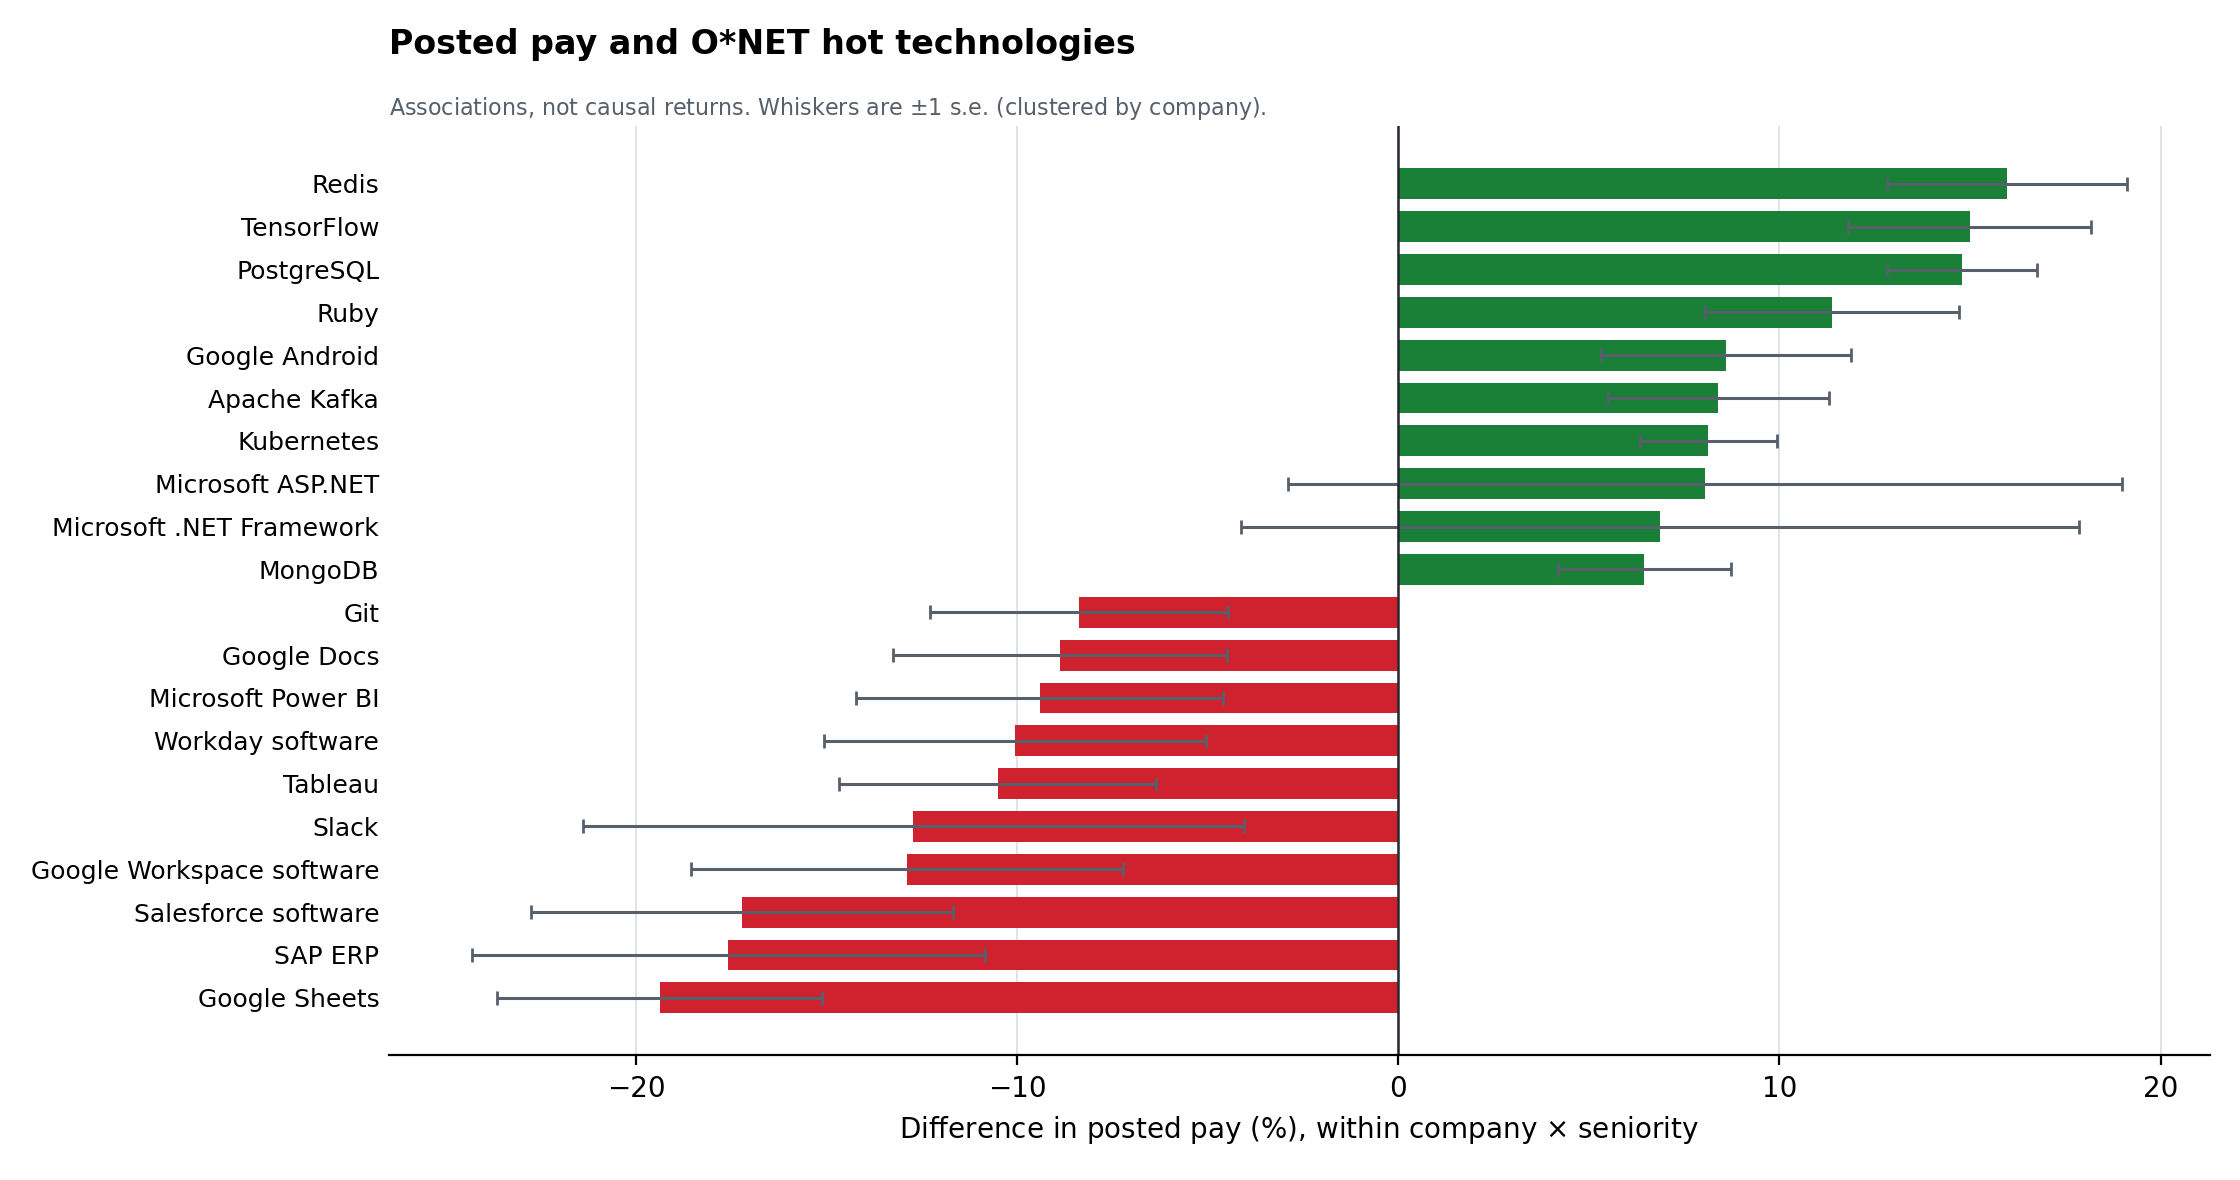
\includegraphics[width=0.88\textwidth,height=0.70\textheight,keepaspectratio]{figs/skill_premia.png}

\vspace{0.2em}
{\footnotesize A hedonic regression: each bar is one skill's price, within firm and seniority.}
\end{frame}

% =============================================================================
\begin{frame}{2. The price of skills}
\begin{wideitemize}
  \item This is a hedonic regression: pay on skill dummies.
  \item Data and infrastructure skills are priced highest.
  \item Office and reporting tools are priced lowest.
  \item A market price, not a causal return: Excel marks admin roles.
\end{wideitemize}
\end{frame}

% =============================================================================
\begin{frame}{3. Does posted pay discount remote work?}
\begin{wideitemize}
  \item Remote work is an amenity: workers value it directly.
  \item If firms priced it in, remote postings would pay less.
  \item Mas and Pallais (2017): workers would give up about 8\% on average.
  \item But their distribution is right-skewed: many value it at zero.
\end{wideitemize}
\end{frame}

% =============================================================================
\begin{frame}{3. Does posted pay discount remote work?}
\centering
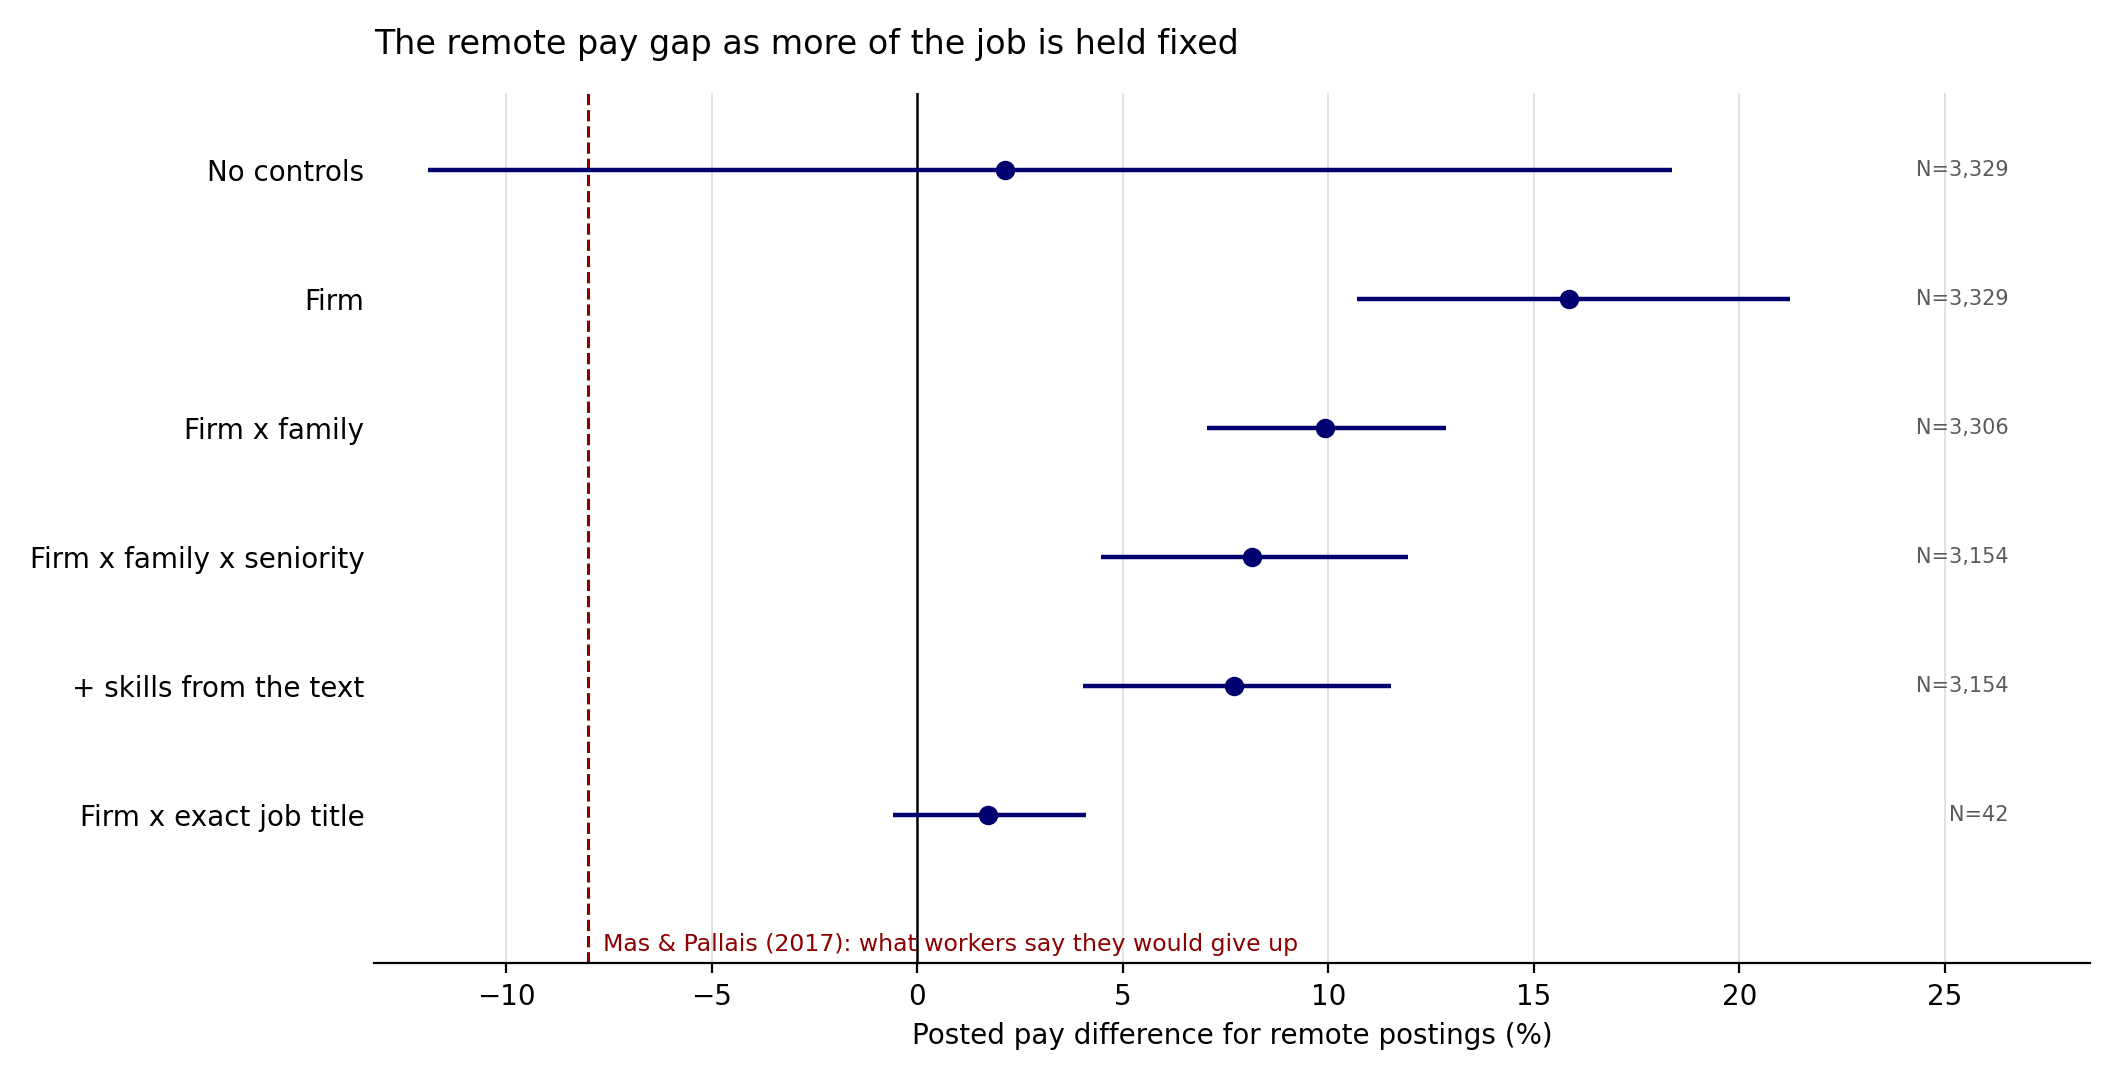
\includegraphics[width=0.92\textwidth,height=0.70\textheight,keepaspectratio]{figs/remote_differential.png}
\end{frame}

% =============================================================================
\begin{frame}{3. Does posted pay discount remote work?}
\begin{wideitemize}
  \item Raw, remote pays more: remote jobs are better jobs.
  \item Hold the title fixed and the gap falls to about zero.
  \item So posted pay does not visibly discount remote.
  \item But this is the posted offer, not agreed pay or workers' value.
  \item So it neither confirms nor refutes the 8\%.
\end{wideitemize}

\vspace{0.6em}
{\footnotesize The tightest comparison rests on 42 postings.}
\end{frame}

\section{Responsibly}
\begin{frame}{Scraping responsibly}
\begin{wideitemize}
  \item Prefer a bulk download or an official API; read robots.txt and the terms.
  \item Identify yourself with a User-Agent, and slow down when you see 429.
  \item Ask for many records per request, not many requests.
  \item Do not collect personal data you do not need.
  \item Keep the raw replies, so results can be reproduced.
\end{wideitemize}
\end{frame}

% =============================================================================
\begin{frame}{What to remember}
\begin{wideitemize}
  \item Look at the page before writing code.
  \item Check for a hidden JSON address before parsing HTML.
  \item Make fewer requests, not faster parsers.
  \item Expect failure, and cache every raw reply.
  \item Collecting the data is the easy part; what you compare is the research.
\end{wideitemize}
\end{frame}

% =============================================================================
% APPENDIX
% =============================================================================
\appendix
\AtBeginSection[]{}
\dividerslide{Appendix}

% =============================================================================
\begin{frame}[fragile]{How the skills were extracted}
\begin{wideitemize}
  \item The list is external: O*NET Hot Technologies, 170 items.
  \item Choosing terms after seeing the results would be circular.
  \item Only requirement sections are read, not company blurb.
  \item Negation is handled, as in this real sentence:
\end{wideitemize}

\begin{lstlisting}[style=code]
"No ML or Research experience is required"
\end{lstlisting}

\begin{wideitemize}
  \item Words like access, cloud and team need the full product name.
\end{wideitemize}
\end{frame}

% =============================================================================
\begin{frame}{A separate question: how is the band set?}
\centering
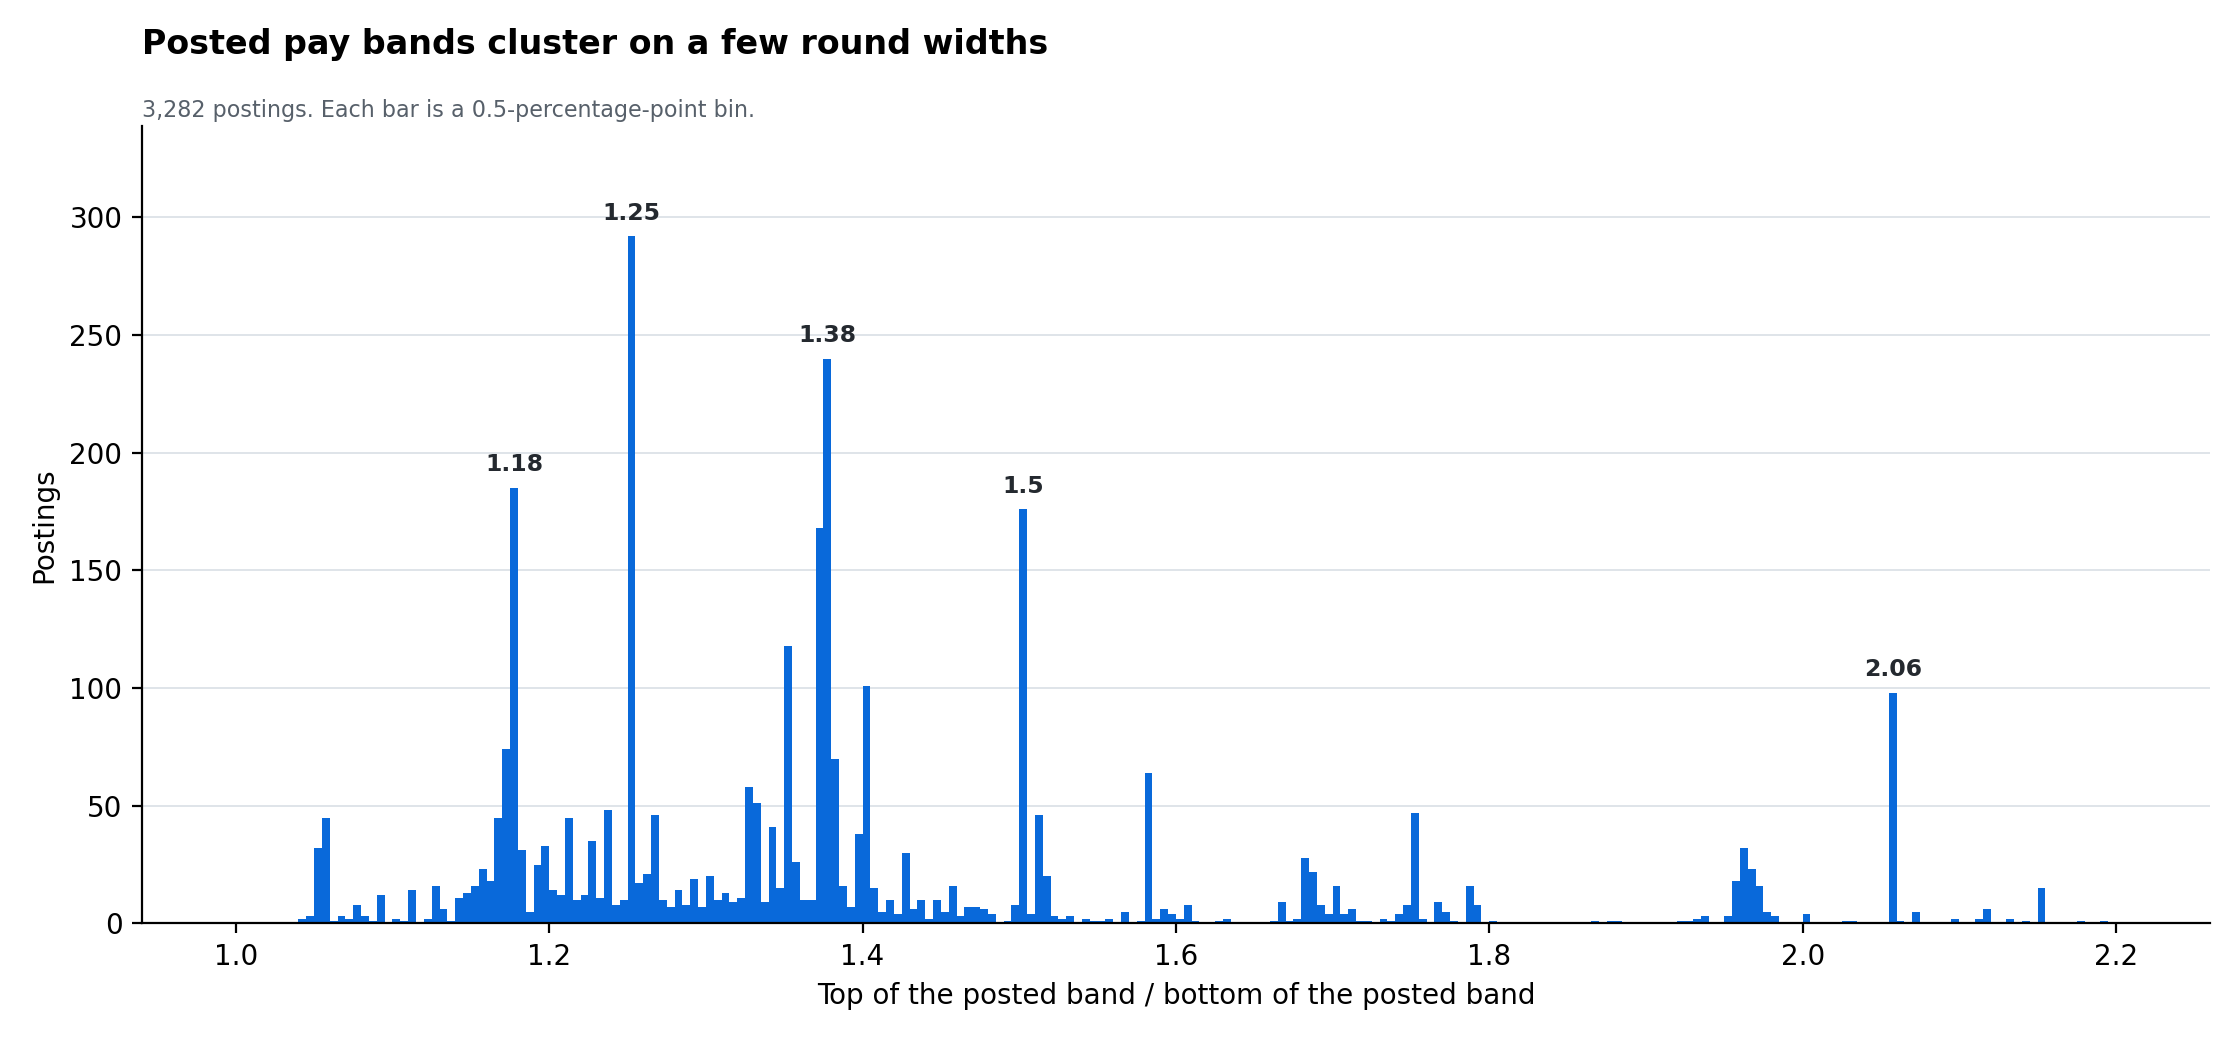
\includegraphics[width=0.92\textwidth,height=0.66\textheight,keepaspectratio]{figs/range_width.png}

\vspace{0.2em}
{\footnotesize Not about attributes and pay --- about how the firm chooses the range.}
\end{frame}

% ============================================================
\begin{frame}{Reading the width result}
\begin{wideitemize}
  \item A band could mean room to negotiate, or a role spanning levels.
  \item It could also be a convention that satisfies a disclosure rule.
  \item Spikes at round ratios point to convention.
  \item A flat percentage is not a flat amount: 31\% of \$400k is \$124k, of \$130k \$40k.
  \item So this says nothing about whether people negotiate.
\end{wideitemize}
\end{frame}

% =============================================================================
\begin{frame}{What this sample is}
\begin{wideitemize}
  \item Firms using one hiring platform, mostly technology.
  \item Only postings that disclose a range.
  \item Advertised pay, not paid pay.
  \item Not the labour market, and not a random sample of it.
\end{wideitemize}
\end{frame}

% =============================================================================
\begin{frame}[fragile]{The false start}
\begin{lstlisting}[style=py]
pat = re.compile(r"\$\s?(\d{1,3}(?:,\d{3})+)\s*-\s*\$\s?(\d{1,3}(?:,\d{3})+)")
\end{lstlisting}

\begin{wideitemize}
  \item Searching the text with a regular expression found 13\% of salaries.
  \item Adding \texttt{?pay\_transparency=true} found 45\%, as typed numbers.
  \item The missing cases were not in the text at all.
  \item Look for structure before writing a regular expression.
\end{wideitemize}
\end{frame}

% =============================================================================
\begin{frame}[fragile]{Politeness in code}
\begin{lstlisting}[style=py]
def get(url, tries=4):
    for attempt in range(tries):
        r = SESSION.get(url, timeout=45)
        if r.status_code == 429:
            time.sleep(2 ** attempt)
            continue
        if r.status_code >= 500:
            time.sleep(1 + attempt)
            continue
        return r
    return None
\end{lstlisting}

\begin{wideitemize}
  \item Wait 1s, then 2s, then 4s before retrying.
  \item Hammering a struggling server is how you get blocked.
\end{wideitemize}
\end{frame}

% =============================================================================
\begin{frame}[fragile]{Reuse the connection}
\begin{columns}[T,onlytextwidth]
  \column{0.46\textwidth}
\begin{lstlisting}[style=py]
for url in urls:
    requests.get(url)
\end{lstlisting}
  \column{0.46\textwidth}
\begin{lstlisting}[style=py]
s = requests.Session()
for url in urls:
    s.get(url)
\end{lstlisting}
\end{columns}

\vspace{0.8em}
\begin{wideitemize}
  \item Each new connection re-negotiates encryption with the server.
  \item A session reuses it, and remembers headers and cookies.
  \item Without this, BeautifulSoup looked slower than Selenium.
\end{wideitemize}
\end{frame}

% =============================================================================
\begin{frame}{Common errors}
\begin{table}
\centering\footnotesize
\begin{tabular}{lp{7.2cm}}
\toprule
Error & Usually means \\
\midrule
\texttt{ModuleNotFoundError}   & installed for a different Python \\
\texttt{JSONDecodeError}       & the reply was not JSON; print \texttt{r.text} \\
\texttt{'NoneType' has no...}  & \texttt{soup.find()} found nothing; the tag changed \\
\texttt{StaleElementReference} & the page rebuilt itself; wait and look again \\
\texttt{SessionNotCreated}     & Selenium older than 4.25, or no Chrome \\
HTTP 403                       & the server refused you; check the terms \\
HTTP 429                       & you are going too fast \\
\bottomrule
\end{tabular}
\end{table}
\end{frame}

% =============================================================================
\begin{frame}{Where to go next}
\begin{wideitemize}
  \item \texttt{playwright}: a faster, more modern Selenium.
  \item \texttt{scrapy}: a framework for large crawls.
  \item Government portals: procurement, courts, transparency registers.
  \item The Internet Archive turns a static site into a historical panel.
  \item Open a page, press F12, and watch the Network tab.
\end{wideitemize}
\end{frame}

\end{document}
